% Mobile ad-hoc network
% Author: Dr. Ludger Humbert
% Source: https://haspe.homeip.net/projekte/ddi/browser/tex/pgf2
\documentclass{standalone}

\usepackage{tikz}
\usepackage{pgf}

\usepackage{xxcolor}

\usetikzlibrary{arrows,shadows,petri}
%                              wg. tokens
\newlength{\imagewidth}
\newlength{\imagescale}

\listfiles



\begin{document}

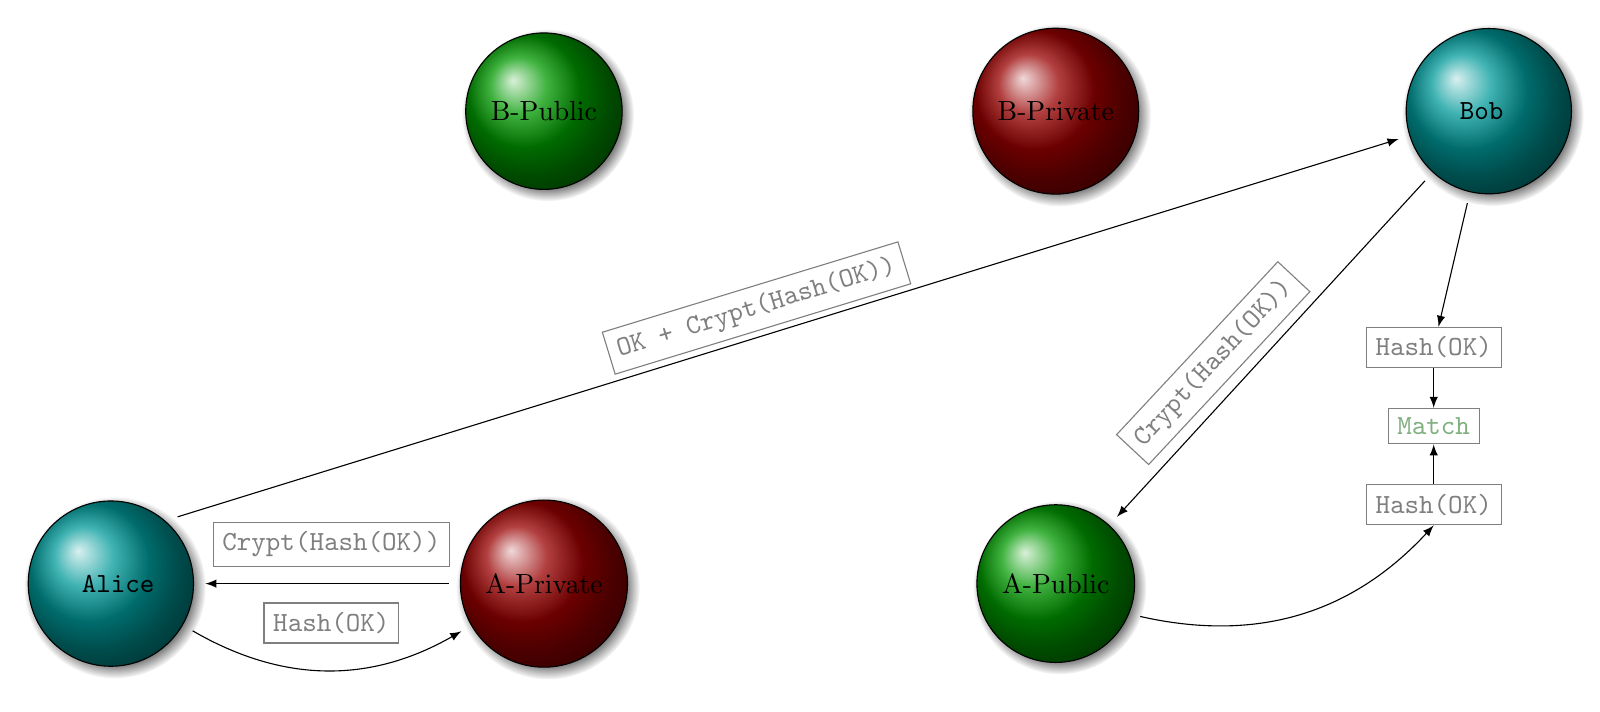
\begin{tikzpicture}[
    knoten/.style={
      shading=ball,
      circle,
      inner sep=.25cm,
      outer sep=.15cm,
      circular drop shadow,
      draw},
    /schriftstueck/.code 2 args={
      \fill[red!50, opacity=#2] #1 rectangle +(.6,.7);
      \foreach \y in {0pt,2pt,4pt,6pt,8pt,10pt,12pt,14pt}
       \draw [yshift=\y, opacity=#2] #1+(0.1,0.1) -- +(0.1,0.1);
      }
    ]

  \node at (0,.5) (knoten0) [knoten, ball color=cyan!60!black] {\texttt{\ \ Alice\ \ }};

  \node[rectangle,draw,opacity=.5] at (2.8,0)  (ack10) {\texttt{Hash(OK)}};
  \node[rectangle,draw,opacity=.5] at (2.8,1)  (ack10) {\texttt{Crypt(Hash(OK))}};
  \node[rectangle,draw,opacity=.5,rotate=17] at (8.2,4)  (ack10) {\texttt{OK + Crypt(Hash(OK))}};

  \node at (5.5,.5) (knoten1) [knoten, ball color=red!60!black] {A-Private};
  \node at (5.5,6.5) (knotenBPublic) [knoten, ball color=green!60!black] {B-Public};



  \node at (12,.5) (knoten2) [knoten, ball color=green!60!black] {A-Public};
  \node at (12,6.5) (knotenBPublic) [knoten, ball color=red!60!black] {B-Private};



  \node at (17.5,6.5) (knoten3) [knoten, ball color=cyan!60!black] {\texttt{\ \ Bob \ \ \ }};
  
  \node[rectangle,draw,opacity=.5,rotate=47] at (14,3.3)  (ack10) {\texttt{Crypt(Hash(OK))}};

  \path  [-latex] (knoten0) edge [bend right] (knoten1);
  \path  [-latex] (knoten1) edge [] (knoten0);
  \path  [-latex] (knoten0.north east) edge [] (knoten3);
  \path  [-latex] (knoten3) edge [] (knoten2);


  \node[rectangle,draw,opacity=.5] at (16.8,3.5)  (ack10) {\texttt{Hash(OK)}};
  \definecolor{dgreen}{RGB}{0, 98, 0}
  \node[rectangle,draw,opacity=.5] at (16.8,2.5)  (ack11) {\texttt{\textcolor{dgreen}{\textbf{Match}}}};
  \node[rectangle,draw,opacity=.5] at (16.8,1.5)  (ack12) {\texttt{Hash(OK)}};


  \path  [-latex] (knoten2) edge [bend right] (ack12.south);
  \path  [-latex] (ack12) edge [] (ack11);

  \path  [-latex] (ack10) edge [] (ack11);

  \path  [-latex] (knoten3) edge [] (ack10);



\end{tikzpicture}

\end{document}
